%
%	Theorieteil
%

\pagebreak
\section{Infrastructure as Code}

\onehalfspacing

\subsection{Terraform}

All major cloud providers have their infrastructure scripting tools, but there's one declarative tool that's available for all infrastructure platforms, on-premise or public, Terraform by HashiCorp.\footnote{See \textit{HashiCorp (2019)}: Deliver infrastructure as code with Terraform. \cite{terraform}}.

As of Rancher 2.3, release in Octover 2012, Rancher has a Terraform provider, and cluster creation and decommissioning can easily be performed from a Terraform plan as part of a move of IT to IaC.\footnote{See \textit{Rancher Labs (2019)}: Introducing the Rancher 2 Terraform Provider. \cite{terraformProvider}}

With Terraform, creating infrastructure becomes as easy as writing a piece of code. Terraform integrates nicely with your existing source code revision systems, such as GitHub or GitLab. It will also make ensure that all infrastructure deployments are repeatable and uniformly executed.

Adding Terraform to the container run-time tool chest of Rancher and Kubernetes is a major benefit and step forward, it will make creation of new Kubernetes clusters so much easier.\footnote{See \textit{Frank, C. (2020)}: Deploy Kubernetes Clusters on Microsoft Azure with Rancher. \cite{deployAzure}}

\subsection{Templates}

Another important piece for your Kubernetes tool chest are templates. Templates will allow you to pre-define certain configuration items across the organization, which will help a lot when dealing with hardening in the next chapter.

Rancher offers templates on a number of levels:

\begin{itemize}
\item Cloud Credentials
\item Node Templates
\item Cluster Templates
\end{itemize}

We'll look at each of these in more detail below, but let's first have a look at the different possibilities of creating a Kubernetes cluster from within Rancher.

\subsection{Cluster Creation}

\subsubsection{Managed Kubernetes}

Overall there are three options to create a Kubernetes cluster with Rancher on any of the big public cloud providers:

\begin{itemize}
\item Managed Kubernetes (GKE, AKS, EKS)
\item Rancher node-driver (Azure, AWS)
\item Custom nodes (GCP, Azure, AWS)
\end{itemize}

To create a managed Kubernetes cluster, you'll have to follow the following steps:

First, within a  Terraform plan, define the Rancher provider. Then, in the Rancher cluster definition, define the GKE, AKS or EKS options and finally have Terraform create the cluster. Terraform will be using the platform API for this.

In this setup, the Kubernetes control plane will be managed by the cloud provider and Rancher's functionality will be somewhat limited.

\subsubsection{Rancher Node-Driver}

If you're happy to have Rancher manage the control plane and have full control, and are on either AWS or Azure, consider using the Rancher node-driver. To do this, following the following steps:

First, within a  Terraform plan, define the Rancher provider. Second, in the Rancher cluster definition, define Azure or AWS cloud provider within the RKE cluster options. Then, create the appropriate cloud credentials and node templates. Finally, have Terraform create the cluster, using docker-machine.

This is the most preferred option, and the one that we will follow throughout the document.

\subsubsection{Custom Nodes}

If you need more fine-grained control over the underlying infrastructure, Rancher also offers the ability to use custom created nodes for its Kubernetes clusters. For this, you'll need to follow these steps:

First, within a  Terraform plan, define both the Rancher provider and an infrastructure provider. Second, in the Rancher cluster definition, define the cloud provider within the RKE cluster options. Then, have Terraform create the cluster nodes with the infrastructure provider and pass the Rancher registration command to cloud-init

Although this is the most flexible approach, Rancher will loose the ability to horizontally scale the node pools, among other features. It also requires that the Terraform plans have access to credentials for the infrastructure provider, which could provide in Rancher centrally in the option above.

\subsubsection{Import}

A fourth, and final option, would be to create clusters completely outside of Terraform and Rancher and import them later. This is a quite valid option, but outside of the scope of our document as it would require other forms of automation.

\subsection{Rancher Provider}

The first step is to set up the credentials for Rancher. All access to Rancher is controlled from the built-in RBAC controller and every use can create their own API keys.

"Picture"

We'll then take the defined token and create the Rancher provider in our \verb|provider.tf| plan file:

\begin{verbatim}
# Rancher
provider "rancher2" {
  api_url = var.rancher-url
  token_key = var.rancher-token
  insecure = true
}
\end{verbatim}

This is all the end-user credentials we'll need to create the Kubernetes clusters.

\subsection{Cloud Credentials}

Text.

\begin{figure}[H]
\centering
\caption {Cloud Credentials}
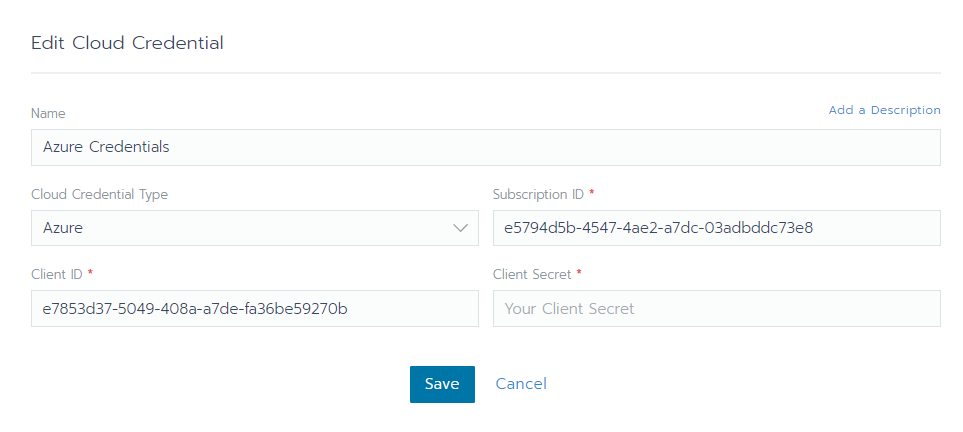
\includegraphics[width=\linewidth]{images/cloud-credentials.png}
\label{fig:cloudCredentials}
\end{figure}

\subsection{Node Templates}

Text. 

\begin{figure}[H]
\centering
\caption {Node Template}
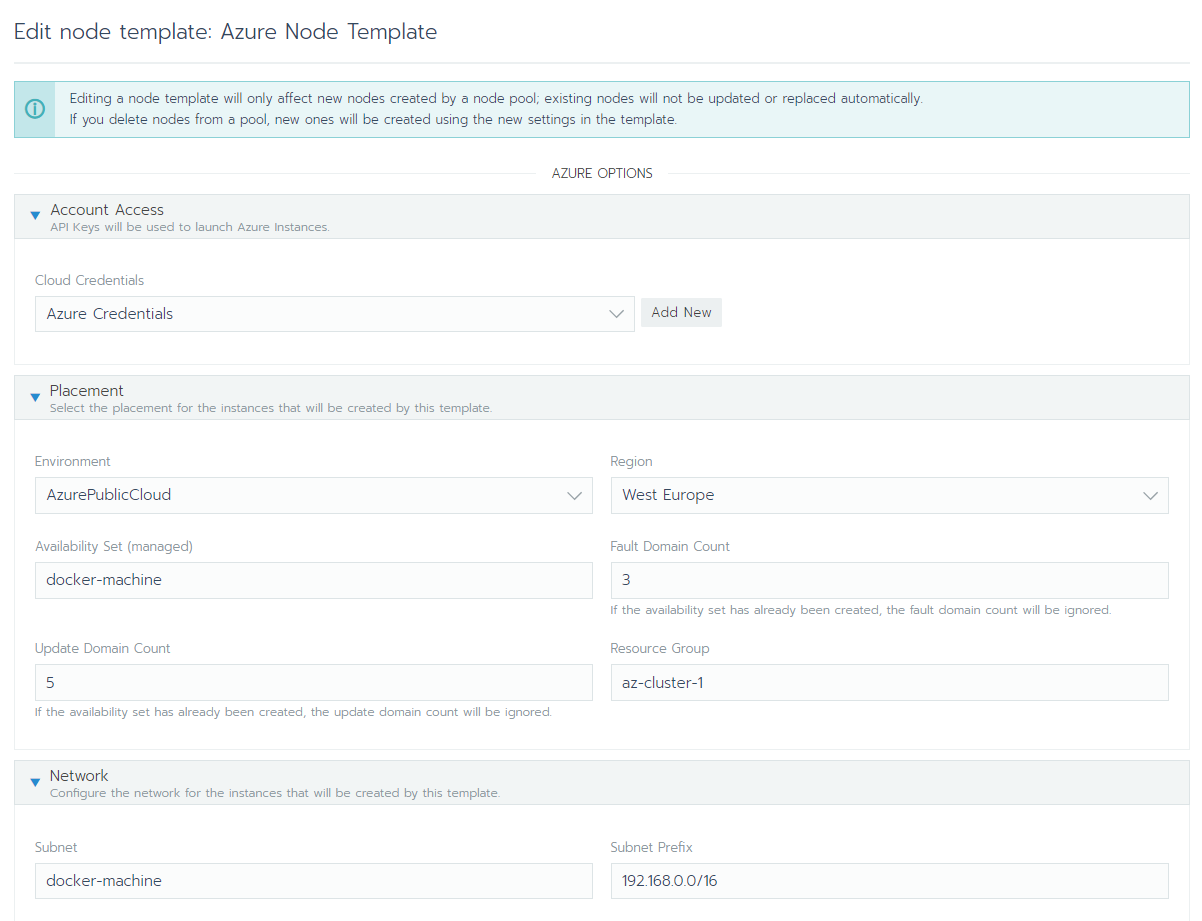
\includegraphics[width=\linewidth]{images/node-template.png}
\label{fig:nodeTemplate}
\end{figure}

\subsection{Cluster Templates}

Text. 

\begin{figure}[H]
\centering
\caption {Cluster Template}
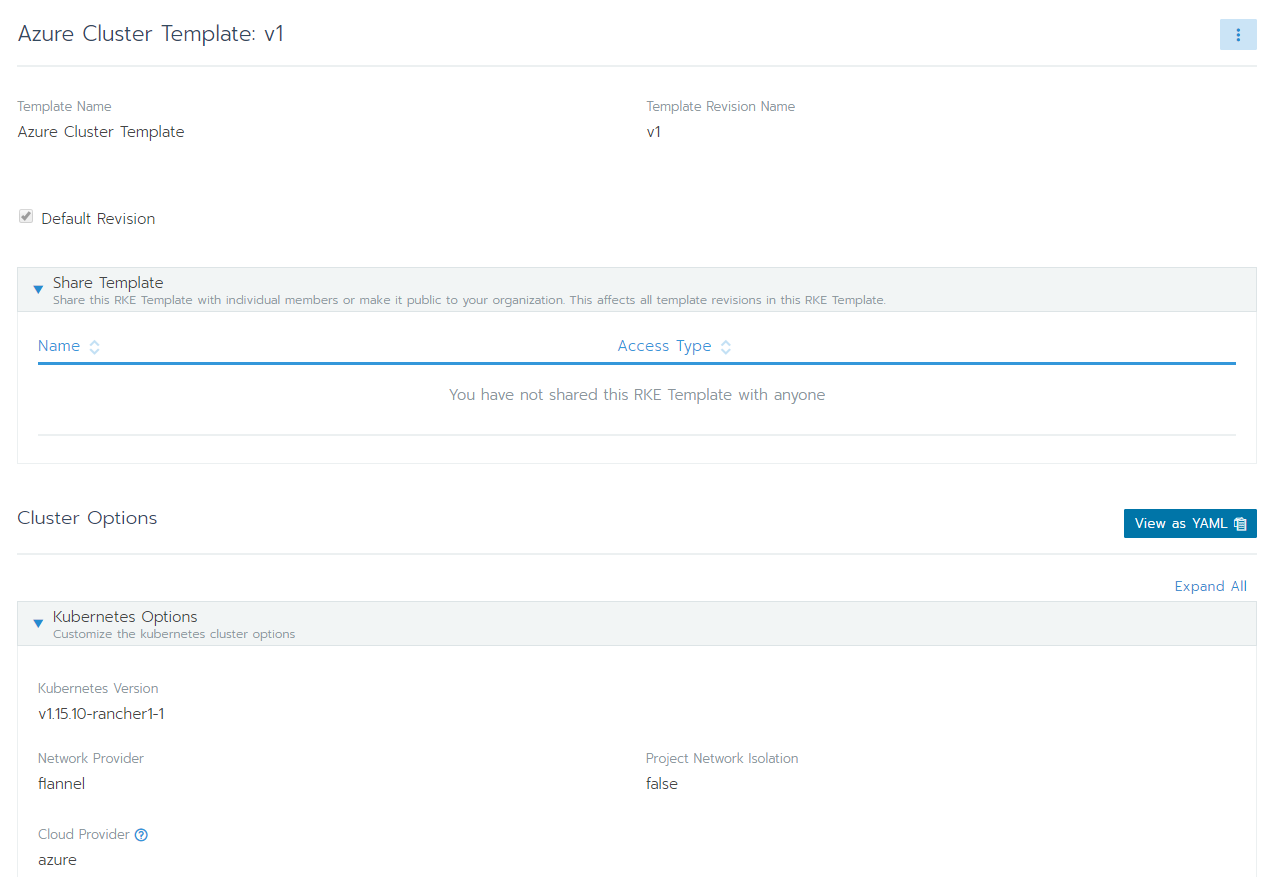
\includegraphics[width=\linewidth]{images/cluster-template.png}
\label{fig:clusterTemplate}
\end{figure}

\subsection{Kubernetes Cluster}

Text. 

\begin{figure}[H]
\centering
\caption {Kubernetes Cluster}
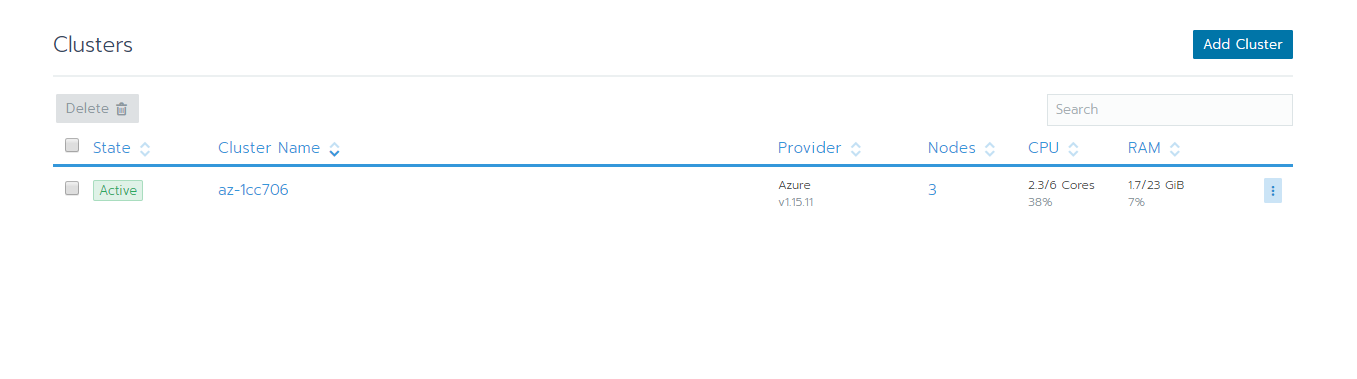
\includegraphics[width=\linewidth]{images/cluster-overview.png}
\label{fig:clusterOverview}
\end{figure}

